\documentclass[12pt]{article}
\usepackage{xeCJK}
\usepackage{graphicx}
\usepackage{amsmath}
\usepackage{enumerate}
\usepackage{diagbox}

\newcommand{\Zmod}{\left|Z\right|}

\begin{document}
\title{数字逻辑设计报告 \quad Music3D组}
\author{潘传宇 \quad 任一}
\maketitle

\newpage
\tableofcontents

\newpage
\section{实验目的}
本实验的最终目的是希望实现一个能够接收音频信号,并将音乐的律动以“立体”的方式显示出来的音频可视化系统。
其中我们使用AN831模块作为音频的输入模块,并使用光立方模块作为“立体s显示”模块。
具体目标有以下几点:
\begin{enumerate}
    \item 实现音频的数字信号输入及处理;
    \item 借助FFT算法实现音频的时域信号向频域信号转换;
    \item 实现频域信号向光立方所需的灯光信号的转换;
    \item 实现灯光信号的“队列式”存储与移位;
    \item 实现灯光信号的“整合打包”与串口协议输出;
\end{enumerate}

\section{实验完成情况与任务分工}
\subsection{完成情况}
\begin{center}
    \begin{tabular}{|c|c|}
        \hline
        时间& 任务\\
        \hline
        第九、十周& 确定主题以及大致设计框架,购买外设,熟悉FPGA板使用\\
        \hline
        第十一周& 确定设计框架,开始编写音频处理部分代码,调试外设\\
        \hline
        第十二周& 完成音频输入、串口输出部分的代码编写,进一步完善设计框架\\
        \hline
        第十三周& 完成音频FFT部分的代码编写,上板调试音频部分\\
        \hline
        第十四周& 完成灯光信号处理部分的代码编写,上板进行整体调试\\
        \hline
        第十五周& 尝试多种模式设计,优化效果\\
        \hline
        第十六周& 准备课堂展示\\
        \hline
    \end{tabular}
\end{center}

\subsection{任务分工}
\begin{itemize}
    \item 潘传宇:调试板子及外设,编写灯光信号处理部分的代码,编写光立方通信协议部分的代码;
    \item 任一: 选购音频模块AN831,编写音频输入及FFT处理部分的代码,协助调试硬件;
\end{itemize}

\section{实验演示说明}
实验演示按照如下步骤进行:
\begin{enumerate}
    \item 按照引脚分配将AN831模块和光立方模块接入FPGA板;
    \item 将板子接入电源,并将程序烧写进入板子;
    \item 启动光立方,通过设置单片机工作模式进入“串口接收模式”;
    \item 烧写完成后,板子立即进入工作状态,此时通过音频线将音频接入AN831模块后,即可看到光立方上随音乐变化的显示效果;
    \item 默认模式为“舒缓模式”,按住实验板上的reset键可进入“动感模式”;
\end{enumerate}
\begin{center}
    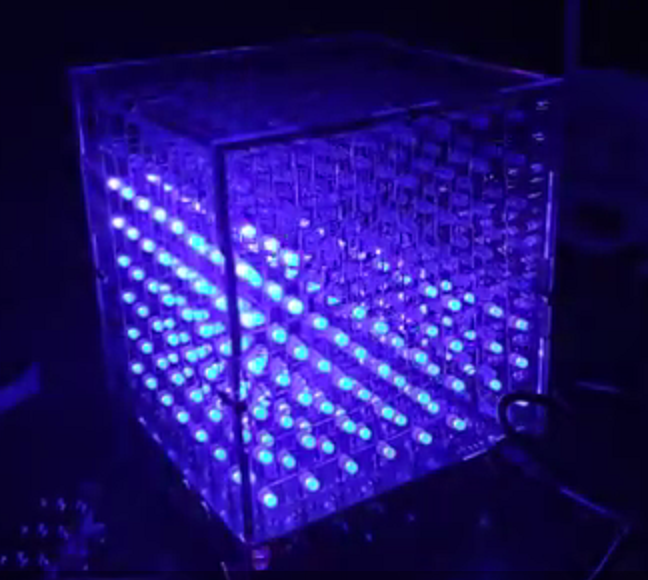
\includegraphics[scale=0.6]{pic/show1.png}
    \\\small{展示效果图}
\end{center}
展示视频链接如下:

\section{文件说明}
\section{总体设计}
\section{关键技术分析}
\subsection{Fast Fourier Transformation}
为了从时域信号中提取频域信息,我们需要使用快速傅里叶变换(FFT)。

在本代码中,我们配置WM8731芯片的采样频率为8KHz, 进行64点的FFT,得到了125Hz, 250Hz, 375Hz, 500Hz, 625Hz, 750Hz, 875Hz, 1000Hz
这8个频率处的频谱分量,正好对应光立方每一帧的8列灯光信息。

为了节约计算成本,我们在进行FFT时,提前通过定点数的方式,储存了旋转因子。

\section{程序注释}
\section{波形仿真结果说明}
\section{遇到问题与解决方法}
\section{实验总结}

\end{document}